\documentclass[10pt,a4paper]{article}
\usepackage[utf8x]{inputenc}
\usepackage[OT2,T1]{fontenc}
%\usepackage{stringenc} % for grffile
\usepackage{ucs}
\usepackage{amsthm} %numéroter les questions
\usepackage[english]{babel}
\usepackage{datetime}
\usepackage{xspace} % typographie IN
\usepackage{hyperref}% hyperliens
\usepackage[all]{hypcap} %lien pointe en haut des figures
\usepackage[english]{varioref} %voir x p y
\usepackage{fancyhdr}% en têtes
%\input cyracc.def
\usepackage[]{graphicx} %include pictures
%\usepackage[encoding,inputencoding=utf8,filenameencoding=utf8]{grffile}
%\usepackage[extendedchars,inputencoding=latin1,filenameencoding=latin1]{grffile}
\usepackage[siunitx ]{circuitikz}
\usepackage{gnuplottex}
\usepackage{ifthen}
\graphicspath{{./figures/}}
%\usepackage{array}
\usepackage{amsmath}
\usepackage[]{xcolor}
\usepackage{tikz}
\usepackage{tikz-timing}
\usetikzlibrary{scopes}
\usetikzlibrary{backgrounds}
\usepackage{listings}
\usepackage{enumitem}
\usepackage[top=1 in, bottom=1 in, left=1.3 in, right=1 in]{geometry} % Yeah, that's bad to play with margins
\usepackage[]{pdfpages}
\usepackage{pdflscape}
\usepackage[]{attachfile}
%\usepackage{colortbl}
%\usepackage{multirow}
\usepackage{booktabs}
\usepackage{makecell}
\usepackage[ ]{subfig}
%\usepackage{rotating}
\usepackage{upgreek}

\newdateformat{mydate}{2013--2014}%hack pour remplacer \THEYEAR

%cyr
%\newcommand\textcyr[1]{{\fontencoding{OT2}\fontfamily{wncyr}\selectfont #1}}
\renewcommand{\marginpar}[1]{} %surcharge pour /marginpar

\newboolean{corrige}
\setboolean{corrige}{true}%corrigé
%\setboolean{corrige}{false}% pas de corrigé

\newboolean{annexes}
%\setboolean{annexes}{true}%annexes
\setboolean{annexes}{false}% pas de annexes

\newboolean{mos}
%\setboolean{mos}{true}%annexes
\setboolean{mos}{false}% pas de annexes

\usepackage{aeguill} %guillemets

%% fancy header & foot
\pagestyle{fancy}
\lhead{[ELEC-H-410] Real-Time Computer Systems Project: Distributed alarm \\}
\rhead{\mydate\today\\ page \thepage} 
\chead{\ifthenelse{\boolean{corrige}}{Corrigé}{}}
\cfoot{}
%%

\pdfinfo{
/Author (Yannick Allard - Raoul Sommeillier, ULB -- BEAMS)
/Title (Project ELEC-H-410, uCOS-II)
/ModDate (D:\pdfdate)
}

\hypersetup{
pdftitle={Project [ELEC-H-410] Real-Time Computer Systems},
pdfauthor={Yannick Allard - Raoul Sommeillier, ©2014 ULB - BEAMS  },
pdfsubject={uCOS-II}
}

\theoremstyle{definition}% questions pas en italique
\newtheorem{E}{\color{blue}Exercise}[] % numéroter les questions [section] ou non []

\newcommand{\reponse}[1]{% pour intégrer une réponse : \reponse{texte} : sera inclus si \boolean{corrige}
	\ifthenelse {\boolean{corrige}} {\paragraph{Réponse :} #1} {}
 }

\newcommand{\addcontentslinenono}[4]{\addtocontents{#1}{\protect\contentsline{#2}{#3}{#4}{}}}

\newcommand{\on}[1]{\operatorname{#1}}

\newcommand{\reg}[1]{\texttt{reg#1}}

\newcommand{\uCOSII}{$\upmu$C/OS-II}

\newcommand{\kw}[1]{\texttt{#1}}

\setlength{\parskip}{1ex plus .5ex minus .5ex} % espacement entre paragraphes
\setlength{\parindent}{0 ex plus 0ex minus 0 ex} % retrait en début de §

\def\labelitemi{--}
\setlist{parsep=0pt,itemsep=0pt,style=standard,leftmargin=\parindent, align=left} % pas d'espace prohibitif entre les items
\setlist{nolistsep}

\newcolumntype{C}[1]{>{\centering\let\newline\\\arraybackslash\hspace{0pt}}m{#1}}

%\setlength{\tabcolsep}{0pt} %no extra space in cells to keep constant tabular width

\date{\vspace{-1cm}\mydate\today}
\title{\vspace{-2cm} Project\\ Real-Time Computer Systems [ELEC-H-410]\\ \textbf{Design a real-time distributed alarm}\ifthenelse{\boolean{corrige}}{~\\Corrigé}{}}

%\author{\vspace{-1cm}}%\textsc{Yannick Allard}}


\lstdefinestyle{customasm}{
 % belowcaptionskip=1\baselineskip,
 % frame=L,
 % xleftmargin=\parindent,
  language=[x86masm]Assembler,
  basicstyle=\footnotesize\ttfamily,
  commentstyle=\itshape\color{purple!40!black},
  comment=[l]//,
}
\lstdefinestyle{customc}{
  belowcaptionskip=1\baselineskip,
  breaklines=true,
  frame=L,
  xleftmargin=\parindent,
  language=C,
  showstringspaces=false,
  basicstyle=\footnotesize\ttfamily,
  keywordstyle=\bfseries\color{green!40!black},
  commentstyle=\itshape\color{purple!40!black},
  identifierstyle=\color{blue},
  stringstyle=\color{orange},
}
\lstset{escapechar=@,style=customc}

\begin{document}

% Introduce a new counter for counting the nodes needed for circling
\newcounter{nodecount}
% Command for making a new node and naming it according to the nodecount counter
\newcommand\tabnode[1]{\addtocounter{nodecount}{1} \tikz \node (\arabic{nodecount}) {#1};}

% Some options common to all the nodes and paths
\tikzstyle{every picture}+=[remember picture,baseline]
\tikzstyle{every node}+=[inner sep=0pt,anchor=base]
\tikzstyle{every path}+=[thick, rounded corners]

% for tikz pict


\maketitle
\section{Purpose}

On the basis of the previous labs you will now create a distributed alarm system working on the CAN network.



\section{Useful documents are stored on the network share:}
 \verb!labo\ELEC-H-410\Useful Documents\!%\marginpar{OK update this}
\texttt{\begin{itemize}
\item dsPIC30F-33F Programmer's Reference.pdf
\item dsPIC33 Data Sheet.pdf section 21
\item Introduction to MPLAB.pdf
\item Explorer 16 User Guide 51589a.pdf
\item MPLAB C30 C Compiler User's guide.pdf
\item uCOSII\_RefMan.pdf
\item Enhanced Controller Area Network.pdf
\item Introduction to language C for microcontrollers.pdf
\item Table of ASCII codes.
\end{itemize}}

%*
%*
%Introduction à MPLAB.pdf*
%*
%La Carte Explorer16.pdf*
%*
%*


\section{Specifications}
In this distributed alarm system, all nodes are equal (i.e. there is not any master node), can work
autonomously but also exchange information through CAN. The application of the node should run under \uCOSII.\\

Each node of the alarm system will have to carry the following functionalities out:
\begin{itemize}
\item Monitor the presence of intruders. %You will have at your disposal an infra-red barrier that
%you can connect to a digital input of the microcontroller.
The sensor will be a push button connected to a digital input of the microcontroller.

\item Arm/disarm the system thanks to a secret code typed on the keyboard. For the moment, you can
use the value B169. Functions to change this code are optional.
\item If an intruder is detected while the system is armed, leave the possibility to disarm the
system using the same code during the first 30s.
\item If the system has not been disarmed within 30s, the alarm should start. You will get a
buzzer or a flashing light that you can connect to an output port.
\end{itemize}

\vspace{0.5cm}

In a distributed system, each node must cooperate with the other members of the network:
\begin{itemize}
\item A node signals its presence when it appears on the network and repeat this message
periodically at least every 5 seconds. This ``heartbeat" enables to detect the disappearance
of the node (failure or sabotage).
\item If a node detects an intrusion, it must signal it so that all other nodes pass in the ``alert"
state, even if they haven't detected anybody.
\item (Dis)arming a node should be propagated to all other nodes; there is no obligation to disarm
at the node which has detected the intrusion.
\item Think about any way to attack your alarm and try to reduce possibilities succeed in doing that.
\end{itemize}

\newpage

To facilitate the management of the communication, we propose that you use the following
protocol:
\begin{itemize}
%\item Each node sends only 1 object (CAN\_ID) between 1 and 254. You need different types of
%messages, the type will be indicated by the data (see Table \ref{Table of messages}).\\
%OR
%\item Each node sends only 1 data (DATA[0]). You need different types of messages, the type will be indicated by 1 object (CAN\_ID) between 1 and 254 that will also define the priority of the message (see Table \ref{Table of messages}).
\item \texttt{Message\_ID} will be fixed during the first brainstorm and is linked to the priority of the messages on the network. Nodes must specify their \texttt{Node\_ID} in the data.
\item The alarm system is limited to 10 nodes whose  \texttt{Node\_ID} is unknown a priori.
\item Then a node boots, it has to find a free identifier, then signal its presence by broadcasting
it regularly.
\end{itemize}

\begin{table} [ht]   %h pour le placement voir vers p110
					\begin{center}
						%Le tableau en tant que tel
						\begin{tabular}{|l|c|c|}
								\hline
								\begin{bf}Message type\end{bf}&\begin{bf}Message\_ID\end{bf}&\begin{bf}Data\end{bf}\\
								\hline
								Heartbeat& 0&node ID\\
								\hline
								Intrusion detected& 1&node ID\\
								\hline
								Node has been armed& 5&node ID\\
								\hline
								Node has been disarmed& 4&node ID\\
								\hline
								Alarm started& 6&node ID\\
								\hline
						\end{tabular}
					\end{center}
					\caption{Table of messages}
					\label{Table of messages}
					\end{table}


\section{Operating mode}

\subsection{Timetable}
Five sessions are dedicated to the project:
\begin{itemize}
\item During the \emph{first project session}, you have to brainstorm about the specifications of a distributed alarm. Don't hesitate to use timing diagrams, block diagrams, state machines  or other operating/functional schemes to share your ideas. You must \textbf{NOT} code anything during this session.
\item During the \emph{next four sessions}, you will use your knowledge and the result of your brainstorming to implement your node of the distributed alarm system. 
\item The \emph{last session} will be split in two times two hours. The first two hours will allow your group to check the effective functioning of your alarm. Your project will be evaluated during the last two hours.
\end{itemize}


\subsection{Evaluation}
The project will we evaluated on the basis of a short presentation of your work and your answers to questions.\\
\textsc{P. Mathys}, \textsc{Y. Allard} and \textsc{R. Sommeillier} will spend several minutes in each group during the last two hours of the last session to check the effective functioning of your alarm, to assess the quality of your code and to ask you a few questions.

\begin{flushright}
\section*{Good luck!}
\end{flushright}

\section{Task splitting}
 \begin{center}
 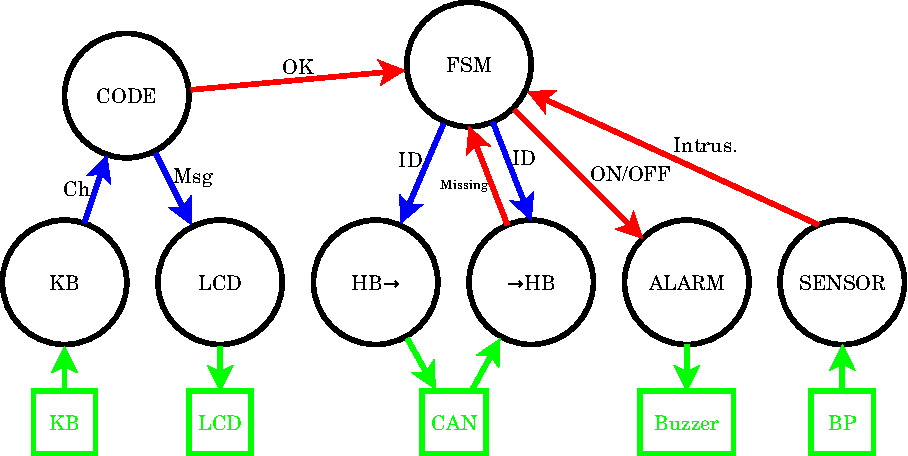
\includegraphics[width=10cm]{taches-crop.pdf}
 \end{center}

\subsection{FSM task: Finite State Machine detail}

\subsection{HB→}
Heartbeat generation

Input: mailbox from FSM with ID

Output: Heartbeat message on the CAN

Behaviour: Periodic message with ID=0, each 5s (max)
\subsection{→HB}
Heartbeat processing

Input: HB messages from the CAN

Input: Mailbox from FSM to add ID in the list

Output: Semaphore to FSM set when ID goes missing on the CAN

Behaviour: Maintains a list with Node ID seen on the CAN. Each message reset a counter for the corresponding NodeID. Periodically, the counter in decremented and when it reaches 0, the semaphore to FSM is set.

All messages can be processed as HB as the Node ID is the first data byte.
\subsection{CODE}
Code input and verification

Input: mailbox from KB

Output: Semaphore to FSM set when valid code

Output: Mailbox: message to display on the LCD, ``*" when char typed, ``Code OK", ``Code wrong"\dots

Behaviour: Based on the char received from KB, send strings to print (stars and/or messages) to the LCD task and set a semaphore to FSM is the code is correct. Reset any partial input after some time.
\subsection{ALARM}
Ring the Alarm

Input: semaphore from FSM

Output: sound on the DAC

Behaviour: When the semaphore is set, play a sound, could use a global variable instead.
\subsection{LCD}
Displays string received from CODE task using a mailbox.

Input: mailbox from CODE

Output: message on the LCD

Behaviour: Reads the content of the mailbox and displays it on the LCD screen.
\subsection{SENSOR}
Detect an intrusion

Input: a push button on the explorer 16 extension board will be used.

Output: set a semaphore to FSM when an intruder is detected

Behaviour: this task sets the semaphore when the button is pushed.

\section{Hardware constraints}
The CAN has several users and so must be protected.


\section{Finite State Machine}
 \begin{center}
 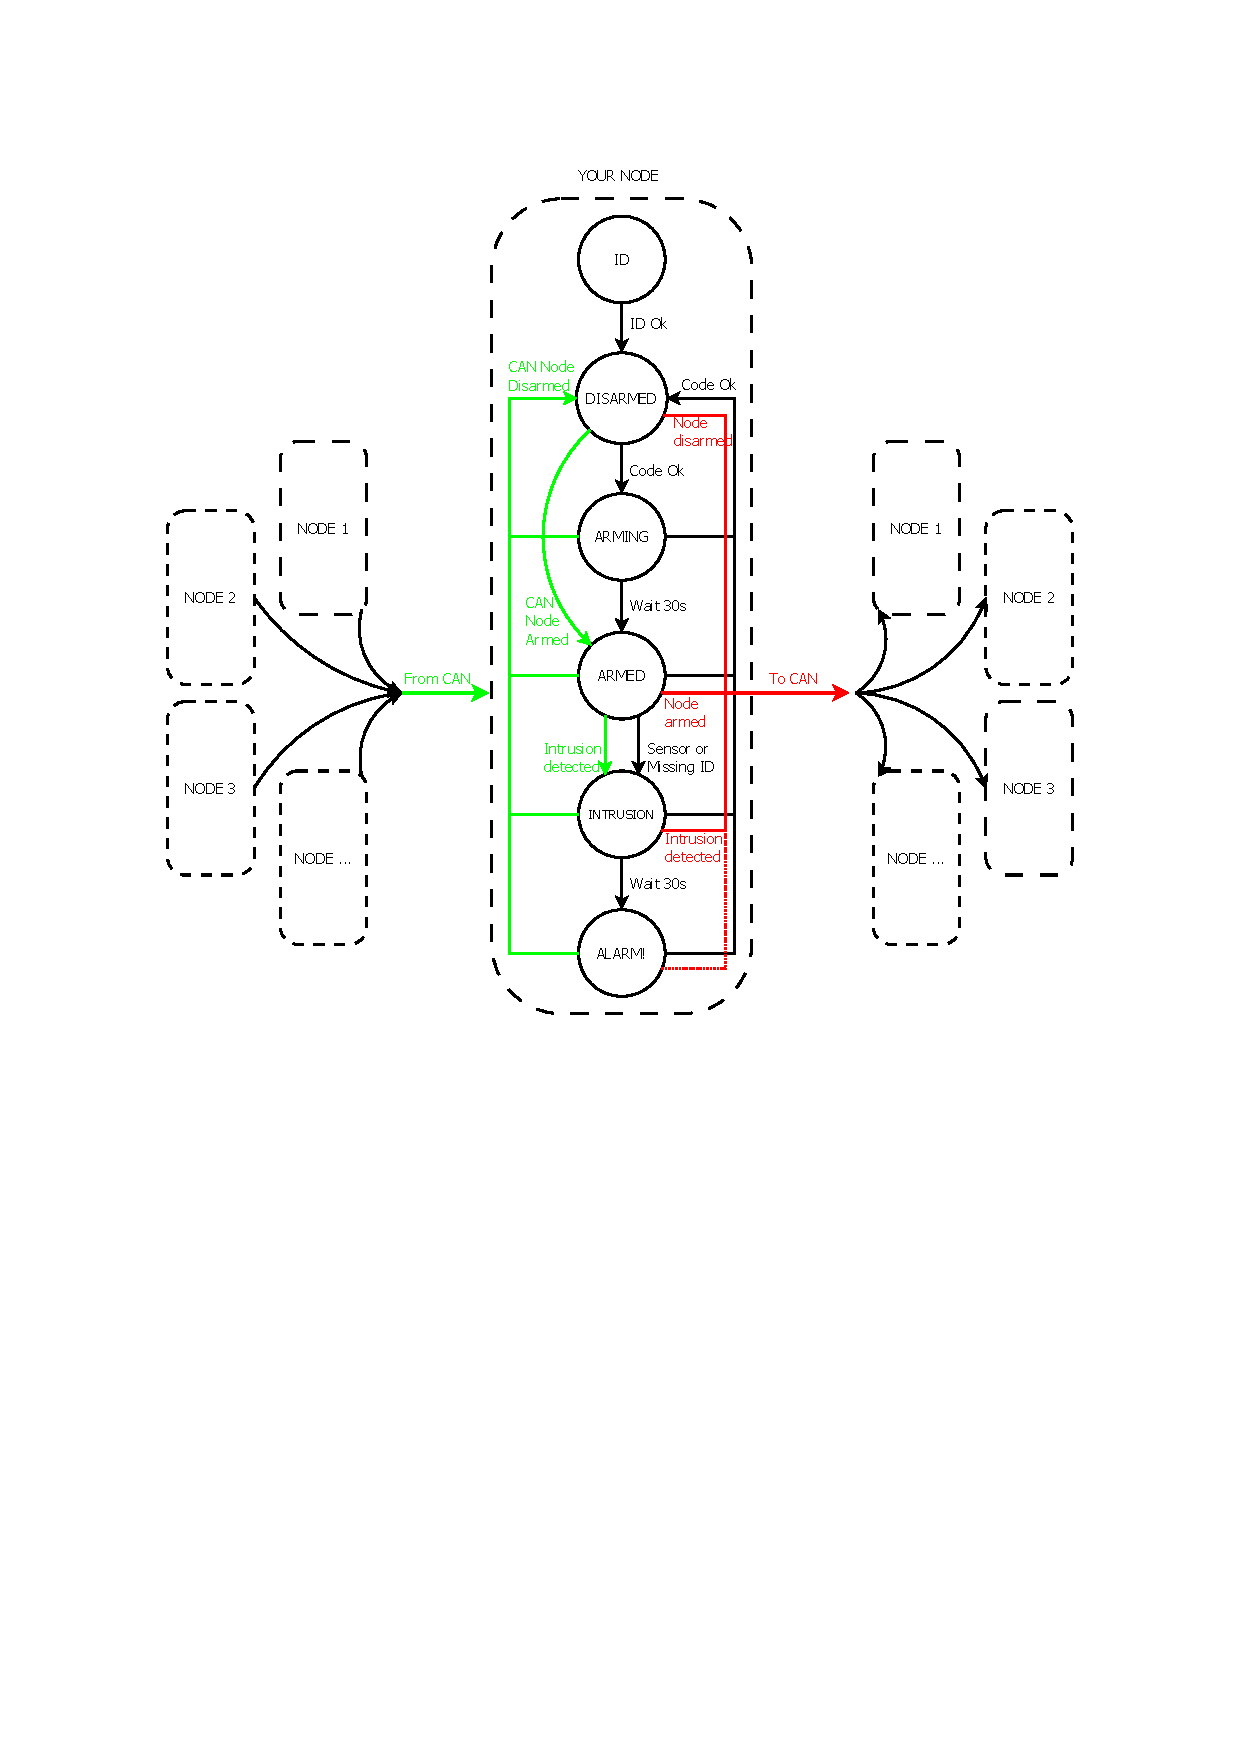
\includegraphics[width=16cm]{FSM_Proj_410.pdf}
 \end{center}

The following diagram represents the finite state machine of your node and its communication with the network. 

\subsection{States of a node}
 \subsubsection{ID}
  Each node of the alarm system must have a CAN\_ID. But this identifier is a priori unknown. Thus, when a node boots, it has firstly to find a free identifier and then signals its presence by broadcasting it regularly (heartbeat message).\\
	
	This state "<ID"> is so the state in which is a node just after booting, i.e. the state of researching a free identifier.\\
	Once this ID is found, the node move from this first state to the following one (DISARMED). 
	
 \subsubsection{DISARMED}
  This state is the one in which the node must be logically as often as possible. The tasks that must be runned into the DISARMED state are to listen to all messages from the CAN and to signal its presence and its state to the other nodes.\\
	
	If the correct arming code is typed on the keyboard on this node, it enters in the ARMING state. And if the node receives via the CAN a message stating "A node has been armed", as all the other nodes, its enter in the ARMED state.\\
		
	When the correct disarming code is type on the keyboard or when the node receives via the CAN, as all the other nodes, a message "A node has been disarmed", the node enters in DISARMED state; whatever was the previous state.
 
 \subsubsection{ARMING}
This state is conceptually a delay of 30s. In practice, it allows the owner of the node (i.e. the house for example) to leave without being detected by the sensor.\\
As previously explained, as for the three next states, if the correct disarming code is pressed on the keyboard or if a disarmed CAN message is received, the node return to the DISARMED state.\\
This state is the only one clearly independant from the network. As a consequence, it is unuseful to communicate the transition towards this state of your node to the other nodes of the network.

 \subsubsection{ARMED}
After waiting 30s, the node enters in the ARMED state and signals this transition to the other nodes.\\
From the ARMED state, the node can pass in INTRUSION state if:
\begin{itemize}
 \item The sensor of the node detects someone. In this case, the node must transmit a "detection message" to the CAN;
 \item If an CAN\_ID from the other nodes that was viewed regularly before via heartbeats messages seems missing (no news during 15 seconds);
 \item If the node received a "detection message" from the CAN. (??????????????? réfléchir là-dessus)
\end{itemize}

 \subsubsection{INTRUSION}
This state is conceptually a delay of 30s. In practice, it allows the owner of the node (i.e. the house for example) to enter, access to the keyboard and type the correct disarming code without triggering the alarm.

\subsubsection{ALARM!}
When entering in this state

\begin{itemize}
 \item{receives informations from the other nodes connected to the network. These received messages should be:}
  \begin{itemize}
	 \item{heartbeat}
	\end{itemize}
 \item{transmits informations to the other nodes connected to the network}
\end{itemize}


\end{document}
